\documentclass{standalone}
\usepackage{tikz}
\usetikzlibrary{patterns, positioning}
\usepackage[sfdefault]{ClearSans} %% option 'sfdefault' activates Clear Sans as the default text font
\usepackage[T1]{fontenc}

\begin{document}
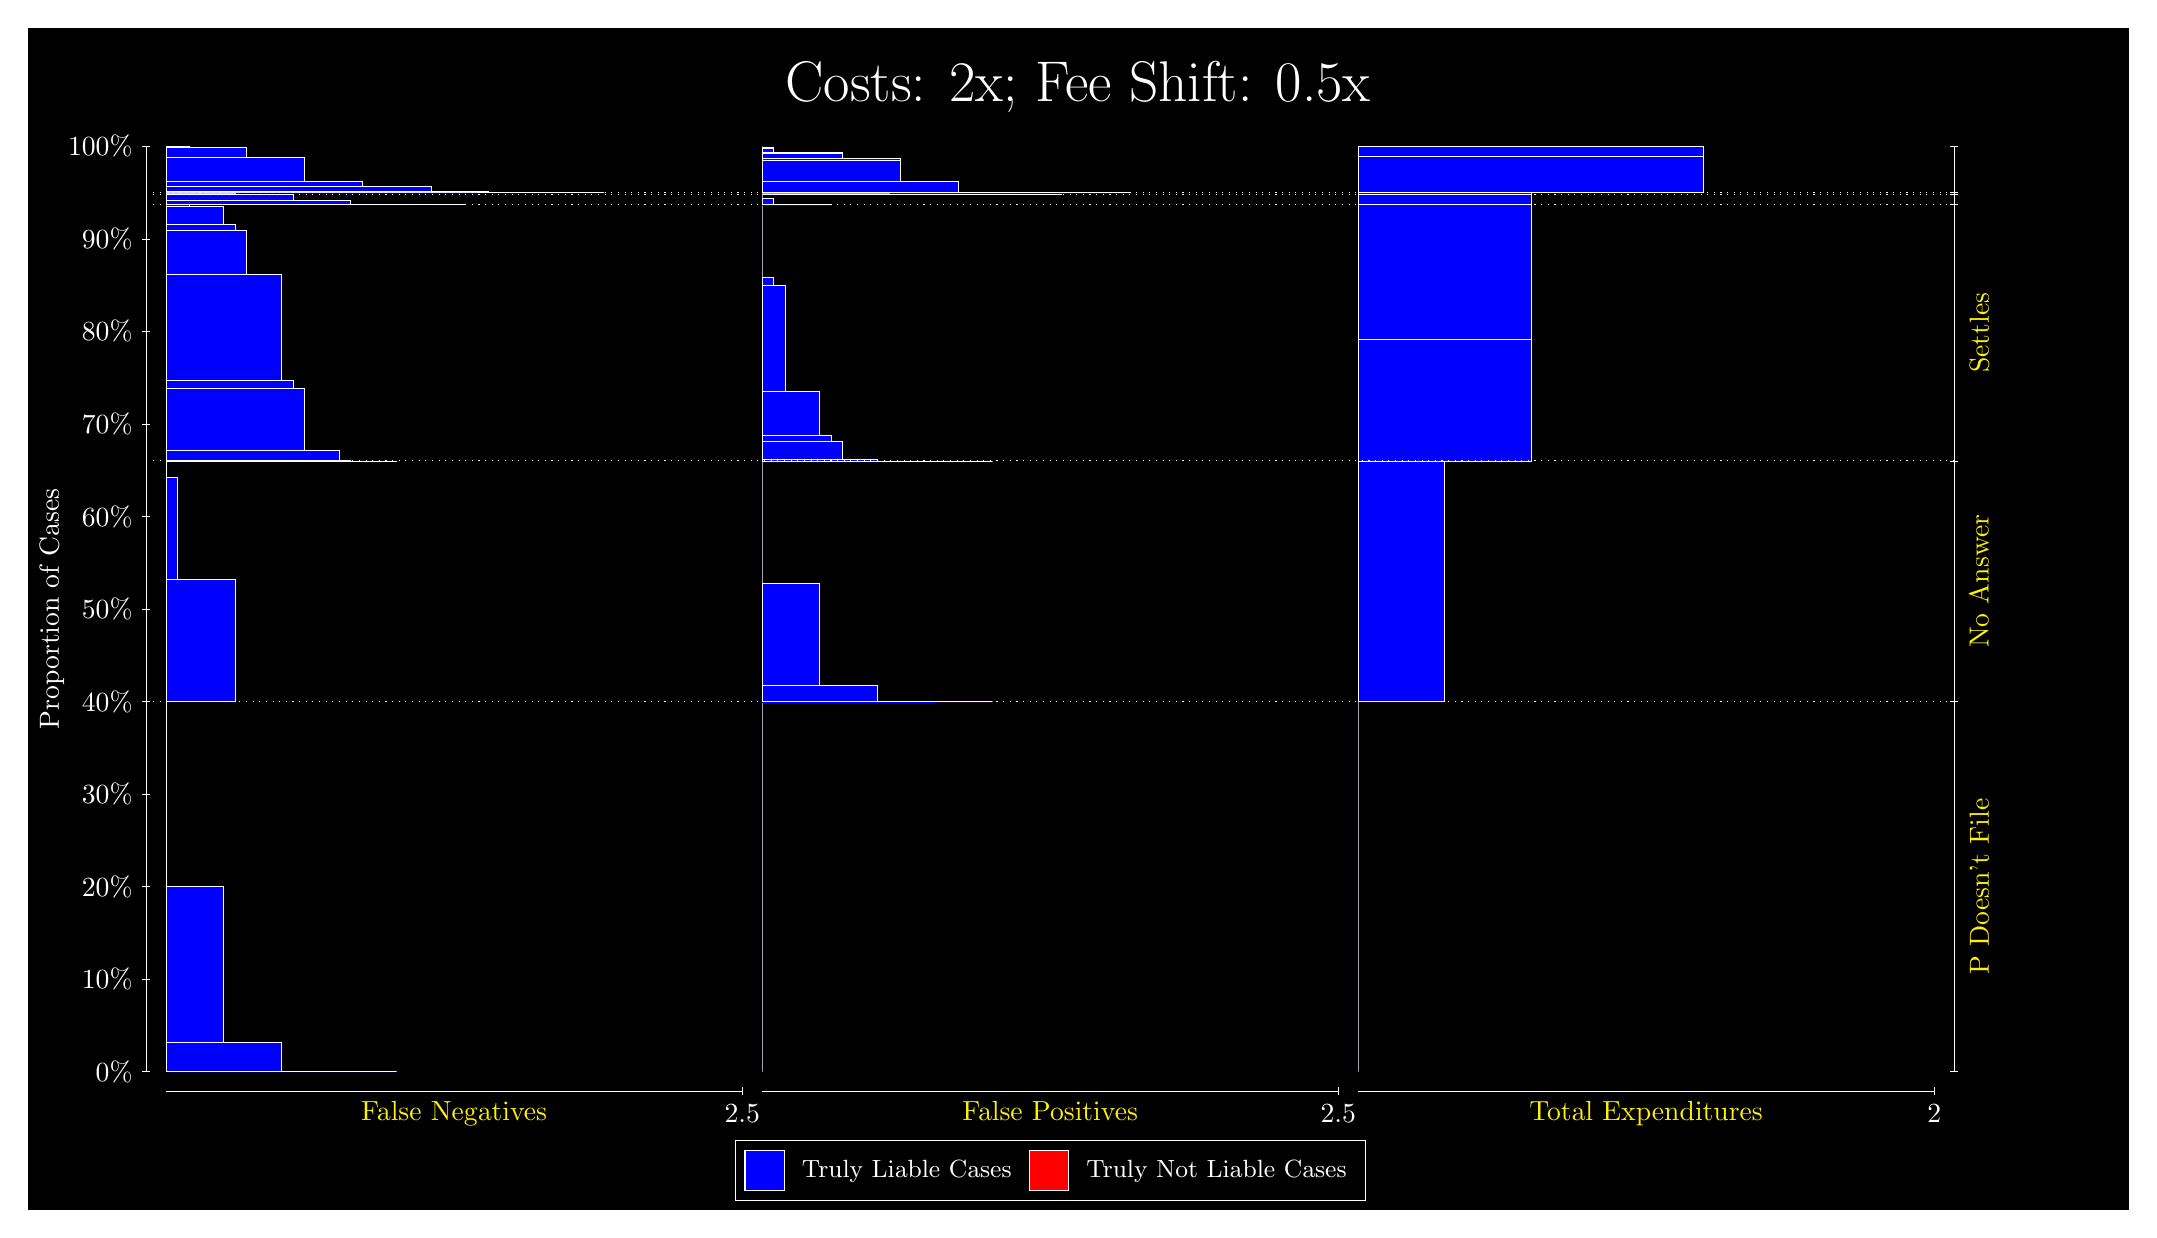
\begin{tikzpicture}
\draw[fill=black] (0,0) rectangle (26.667,15);
\draw[text=white] (0,13.5) rectangle (26.667,15) node[midway] {\huge Costs: 2x; Fee Shift: 0.5x};
\draw[white, very thin] (1.5,1.75) -- (1.5,13.5);
\node[rotate=90, text=white, anchor=center] at (0.3, 7.625) {Proportion of Cases};
\draw[white, very thin] (1.45,1.75) -- (1.55,1.75);
\node[text=white, anchor=east] at (1.45, 1.75) {0\%};
\draw[white, very thin] (1.45,2.925) -- (1.55,2.925);
\node[text=white, anchor=east] at (1.45, 2.925) {10\%};
\draw[white, very thin] (1.45,4.1) -- (1.55,4.1);
\node[text=white, anchor=east] at (1.45, 4.1) {20\%};
\draw[white, very thin] (1.45,5.275) -- (1.55,5.275);
\node[text=white, anchor=east] at (1.45, 5.275) {30\%};
\draw[white, very thin] (1.45,6.45) -- (1.55,6.45);
\node[text=white, anchor=east] at (1.45, 6.45) {40\%};
\draw[white, very thin] (1.45,7.625) -- (1.55,7.625);
\node[text=white, anchor=east] at (1.45, 7.625) {50\%};
\draw[white, very thin] (1.45,8.8) -- (1.55,8.8);
\node[text=white, anchor=east] at (1.45, 8.8) {60\%};
\draw[white, very thin] (1.45,9.975) -- (1.55,9.975);
\node[text=white, anchor=east] at (1.45, 9.975) {70\%};
\draw[white, very thin] (1.45,11.15) -- (1.55,11.15);
\node[text=white, anchor=east] at (1.45, 11.15) {80\%};
\draw[white, very thin] (1.45,12.325) -- (1.55,12.325);
\node[text=white, anchor=east] at (1.45, 12.325) {90\%};
\draw[white, very thin] (1.45,13.5) -- (1.55,13.5);
\node[text=white, anchor=east] at (1.45, 13.5) {100\%};

\draw[white, very thin] (24.457,1.75) -- (24.457,13.5);
\draw[white, very thin] (24.407,1.75) -- (24.507,1.75);
\node[anchor=west] at (24.407, 1.75) {};
\draw[white, very thin] (24.407,6.4489) -- (24.507,6.4489);
\node[anchor=west] at (24.407, 6.4489) {};
\draw[white, very thin] (24.407,9.5049) -- (24.507,9.5049);
\node[anchor=west] at (24.407, 9.5049) {};
\draw[white, very thin] (24.407,12.76) -- (24.507,12.76);
\node[anchor=west] at (24.407, 12.76) {};
\draw[white, very thin] (24.407,12.893) -- (24.507,12.893);
\node[anchor=west] at (24.407, 12.893) {};
\draw[white, very thin] (24.407,12.912) -- (24.507,12.912);
\node[anchor=west] at (24.407, 12.912) {};
\draw[white, very thin] (24.407,13.5) -- (24.507,13.5);
\node[anchor=west] at (24.407, 13.5) {};

\draw[white, very thin, fill=blue] (1.75,1.75) rectangle (4.6775,1.75);
\draw[white, very thin, fill=blue] (1.75,1.75) rectangle (3.9457,1.7532);
\draw[white, very thin, fill=blue] (1.75,1.7532) rectangle (3.2138,2.126);
\draw[white, very thin, fill=blue] (1.75,2.126) rectangle (2.4819,4.1027);
\draw[white, very thin, fill=red] (1.75,4.1027) rectangle (1.75,4.1027);
\draw[white, very thin, fill=blue] (1.75,4.1027) rectangle (1.75,6.4489);
\draw[white, very thin, fill=blue] (1.75,6.4489) rectangle (2.6283,8.0068);
\draw[white, very thin, fill=blue] (1.75,8.0068) rectangle (1.8964,9.2999);
\draw[white, very thin, fill=red] (1.75,9.2999) rectangle (1.75,9.2999);
\draw[white, very thin, fill=blue] (1.75,9.2999) rectangle (1.75,9.5049);
\draw[white, very thin, fill=blue] (1.75,9.5049) rectangle (4.6775,9.5056);
\draw[white, very thin, fill=blue] (1.75,9.5056) rectangle (4.092,9.5068);
\draw[white, very thin, fill=blue] (1.75,9.5068) rectangle (3.9457,9.6443);
\draw[white, very thin, fill=blue] (1.75,9.6443) rectangle (3.5065,10.425);
\draw[white, very thin, fill=blue] (1.75,10.425) rectangle (3.3602,10.529);
\draw[white, very thin, fill=blue] (1.75,10.529) rectangle (3.2138,11.874);
\draw[white, very thin, fill=blue] (1.75,11.874) rectangle (2.7746,12.428);
\draw[white, very thin, fill=blue] (1.75,12.428) rectangle (2.6283,12.513);
\draw[white, very thin, fill=blue] (1.75,12.513) rectangle (2.4819,12.739);
\draw[white, very thin, fill=blue] (1.75,12.739) rectangle (2.0428,12.759);
\draw[white, very thin, fill=blue] (1.75,12.759) rectangle (1.8964,12.759);
\draw[white, very thin, fill=red] (1.75,12.759) rectangle (1.75,12.759);
\draw[white, very thin, fill=blue] (1.75,12.759) rectangle (1.75,12.76);
\draw[white, very thin, fill=blue] (1.75,12.76) rectangle (5.5558,12.76);
\draw[white, very thin, fill=blue] (1.75,12.76) rectangle (4.8239,12.76);
\draw[white, very thin, fill=blue] (1.75,12.76) rectangle (4.092,12.809);
\draw[white, very thin, fill=blue] (1.75,12.809) rectangle (3.3602,12.891);
\draw[white, very thin, fill=blue] (1.75,12.891) rectangle (2.6283,12.893);
\draw[white, very thin, fill=red] (1.75,12.893) rectangle (1.75,12.893);
\draw[white, very thin, fill=blue] (1.75,12.893) rectangle (2.6283,12.899);
\draw[white, very thin, fill=blue] (1.75,12.899) rectangle (1.8964,12.912);
\draw[white, very thin, fill=red] (1.75,12.912) rectangle (1.75,12.912);
\draw[white, very thin, fill=blue] (1.75,12.912) rectangle (1.75,12.912);
\draw[white, very thin, fill=blue] (1.75,12.912) rectangle (7.3123,12.912);
\draw[white, very thin, fill=blue] (1.75,12.912) rectangle (6.5805,12.912);
\draw[white, very thin, fill=blue] (1.75,12.912) rectangle (5.8486,12.924);
\draw[white, very thin, fill=blue] (1.75,12.924) rectangle (5.7022,12.924);
\draw[white, very thin, fill=blue] (1.75,12.924) rectangle (5.1167,12.989);
\draw[white, very thin, fill=blue] (1.75,12.989) rectangle (4.9703,12.989);
\draw[white, very thin, fill=blue] (1.75,12.989) rectangle (4.3848,12.99);
\draw[white, very thin, fill=blue] (1.75,12.99) rectangle (4.2384,13.062);
\draw[white, very thin, fill=blue] (1.75,13.062) rectangle (3.6529,13.062);
\draw[white, very thin, fill=blue] (1.75,13.062) rectangle (3.5065,13.356);
\draw[white, very thin, fill=blue] (1.75,13.356) rectangle (2.7746,13.492);
\draw[white, very thin, fill=blue] (1.75,13.492) rectangle (2.0428,13.5);
\draw[white, very thin, fill=red] (1.75,13.5) rectangle (1.75,13.5);
\draw[white, very thin, fill=blue] (1.75,13.5) rectangle (1.75,13.5);
\draw[white, very thin, fill=red] (9.3189,1.75) rectangle (9.3189,1.75);
\draw[white, very thin, fill=blue] (9.3189,1.75) rectangle (9.3189,6.4489);
\draw[white, very thin, fill=red] (9.3189,6.4489) rectangle (12.246,6.4489);
\draw[white, very thin, fill=blue] (9.3189,6.4489) rectangle (12.246,6.4489);
\draw[white, very thin, fill=blue] (9.3189,6.4489) rectangle (11.515,6.4493);
\draw[white, very thin, fill=blue] (9.3189,6.4493) rectangle (10.783,6.654);
\draw[white, very thin, fill=blue] (9.3189,6.654) rectangle (10.051,7.9471);
\draw[white, very thin, fill=blue] (9.3189,7.9471) rectangle (9.3189,9.5049);
\draw[white, very thin, fill=red] (9.3189,9.5049) rectangle (12.246,9.5049);
\draw[white, very thin, fill=blue] (9.3189,9.5049) rectangle (12.246,9.5049);
\draw[white, very thin, fill=red] (9.3189,9.5049) rectangle (11.661,9.5049);
\draw[white, very thin, fill=blue] (9.3189,9.5049) rectangle (11.661,9.5049);
\draw[white, very thin, fill=blue] (9.3189,9.5049) rectangle (11.515,9.5049);
\draw[white, very thin, fill=red] (9.3189,9.5049) rectangle (11.075,9.5049);
\draw[white, very thin, fill=blue] (9.3189,9.5049) rectangle (11.075,9.5054);
\draw[white, very thin, fill=blue] (9.3189,9.5054) rectangle (10.929,9.5055);
\draw[white, very thin, fill=blue] (9.3189,9.5055) rectangle (10.783,9.5253);
\draw[white, very thin, fill=blue] (9.3189,9.5253) rectangle (10.344,9.7516);
\draw[white, very thin, fill=blue] (9.3189,9.7516) rectangle (10.197,9.8364);
\draw[white, very thin, fill=blue] (9.3189,9.8364) rectangle (10.051,10.391);
\draw[white, very thin, fill=blue] (9.3189,10.391) rectangle (9.6116,11.736);
\draw[white, very thin, fill=blue] (9.3189,11.736) rectangle (9.4652,11.839);
\draw[white, very thin, fill=blue] (9.3189,11.839) rectangle (9.3189,12.76);
\draw[white, very thin, fill=red] (9.3189,12.76) rectangle (10.197,12.76);
\draw[white, very thin, fill=blue] (9.3189,12.76) rectangle (10.197,12.761);
\draw[white, very thin, fill=blue] (9.3189,12.761) rectangle (9.4652,12.843);
\draw[white, very thin, fill=blue] (9.3189,12.843) rectangle (9.3189,12.893);
\draw[white, very thin, fill=red] (9.3189,12.893) rectangle (13.125,12.893);
\draw[white, very thin, fill=blue] (9.3189,12.893) rectangle (13.125,12.893);
\draw[white, very thin, fill=blue] (9.3189,12.893) rectangle (12.393,12.893);
\draw[white, very thin, fill=blue] (9.3189,12.893) rectangle (11.661,12.893);
\draw[white, very thin, fill=blue] (9.3189,12.893) rectangle (10.929,12.906);
\draw[white, very thin, fill=blue] (9.3189,12.906) rectangle (10.197,12.912);
\draw[white, very thin, fill=red] (9.3189,12.912) rectangle (14.003,12.912);
\draw[white, very thin, fill=blue] (9.3189,12.912) rectangle (14.003,12.912);
\draw[white, very thin, fill=red] (9.3189,12.912) rectangle (13.271,12.912);
\draw[white, very thin, fill=blue] (9.3189,12.912) rectangle (13.271,12.912);
\draw[white, very thin, fill=red] (9.3189,12.912) rectangle (12.539,12.912);
\draw[white, very thin, fill=blue] (9.3189,12.912) rectangle (12.539,12.92);
\draw[white, very thin, fill=blue] (9.3189,12.92) rectangle (11.807,13.055);
\draw[white, very thin, fill=red] (9.3189,13.055) rectangle (11.807,13.055);
\draw[white, very thin, fill=blue] (9.3189,13.055) rectangle (11.807,13.056);
\draw[white, very thin, fill=blue] (9.3189,13.056) rectangle (11.075,13.318);
\draw[white, very thin, fill=blue] (9.3189,13.318) rectangle (11.075,13.35);
\draw[white, very thin, fill=red] (9.3189,13.35) rectangle (10.929,13.35);
\draw[white, very thin, fill=blue] (9.3189,13.35) rectangle (10.929,13.35);
\draw[white, very thin, fill=blue] (9.3189,13.35) rectangle (10.344,13.408);
\draw[white, very thin, fill=blue] (9.3189,13.408) rectangle (10.344,13.422);
\draw[white, very thin, fill=blue] (9.3189,13.422) rectangle (10.197,13.423);
\draw[white, very thin, fill=red] (9.3189,13.423) rectangle (10.197,13.423);
\draw[white, very thin, fill=blue] (9.3189,13.423) rectangle (10.197,13.423);
\draw[white, very thin, fill=blue] (9.3189,13.423) rectangle (9.6116,13.424);
\draw[white, very thin, fill=blue] (9.3189,13.424) rectangle (9.6116,13.424);
\draw[white, very thin, fill=blue] (9.3189,13.424) rectangle (9.4652,13.473);
\draw[white, very thin, fill=blue] (9.3189,13.473) rectangle (9.4652,13.488);
\draw[white, very thin, fill=blue] (9.3189,13.488) rectangle (9.3189,13.5);
\draw[white, very thin, fill=red] (16.888,1.75) rectangle (16.888,1.75);
\draw[white, very thin, fill=blue] (16.888,1.75) rectangle (16.888,6.4489);
\draw[white, very thin, fill=red] (16.888,6.4489) rectangle (17.986,6.4489);
\draw[white, very thin, fill=blue] (16.888,6.4489) rectangle (17.986,9.5049);
\draw[white, very thin, fill=red] (16.888,9.5049) rectangle (19.083,9.5049);
\draw[white, very thin, fill=blue] (16.888,9.5049) rectangle (19.083,11.05);
\draw[white, very thin, fill=red] (16.888,11.05) rectangle (19.083,11.05);
\draw[white, very thin, fill=blue] (16.888,11.05) rectangle (19.083,12.76);
\draw[white, very thin, fill=red] (16.888,12.76) rectangle (19.083,12.76);
\draw[white, very thin, fill=blue] (16.888,12.76) rectangle (19.083,12.893);
\draw[white, very thin, fill=red] (16.888,12.893) rectangle (19.083,12.893);
\draw[white, very thin, fill=blue] (16.888,12.893) rectangle (19.083,12.912);
\draw[white, very thin, fill=red] (16.888,12.912) rectangle (21.279,12.912);
\draw[white, very thin, fill=blue] (16.888,12.912) rectangle (21.279,13.376);
\draw[white, very thin, fill=red] (16.888,13.376) rectangle (21.279,13.376);
\draw[white, very thin, fill=blue] (16.888,13.376) rectangle (21.279,13.5);
\draw[white, dotted] (1.5,6.4489) -- (24.457,6.4489);
\draw[white, dotted] (1.5,9.5049) -- (24.457,9.5049);
\draw[white, dotted] (1.5,12.76) -- (24.457,12.76);
\draw[white, dotted] (1.5,12.893) -- (24.457,12.893);
\draw[white, dotted] (1.5,12.912) -- (24.457,12.912);
\draw[white, very thin] (1.75,1.5) -- (9.0689,1.5);
\node[text=yellow, anchor=north] at (5.4094, 1.5) {False Negatives};
\draw[white, very thin] (9.0689,1.45) -- (9.0689,1.55);
\node[text=white, anchor=north] at (9.0689, 1.45) {2.5};

\draw[white, very thin] (9.3189,1.5) -- (16.638,1.5);
\node[text=yellow, anchor=north] at (12.978, 1.5) {False Positives};
\draw[white, very thin] (16.638,1.45) -- (16.638,1.55);
\node[text=white, anchor=north] at (16.638, 1.45) {2.5};

\draw[white, very thin] (16.888,1.5) -- (24.207,1.5);
\node[text=yellow, anchor=north] at (20.547, 1.5) {Total Expenditures};
\draw[white, very thin] (24.207,1.45) -- (24.207,1.55);
\node[text=white, anchor=north] at (24.207, 1.45) {2};

\node[text=yellow, centered, rotate=90] at (24.777, 4.0995) {P Doesn't File};
\node[text=yellow, centered, rotate=90] at (24.777, 7.9769) {No Answer};
\node[text=yellow, centered, rotate=90] at (24.777, 11.132) {Settles};




\draw (12.978300999999998,1.5) node[draw=none] (baseCoordinate) {};
\begin{scope}[align=center]
        \matrix[scale=0.5, draw=white, below=0.5cm of baseCoordinate, nodes={draw}, column sep=0.1cm]{
            \node[rectangle, draw, minimum width=0.5cm, minimum height=0.5cm, fill=blue] {}; &
            \node[draw=none, font=\small, text=white] (B) {Truly Liable Cases}; &
            \node[rectangle, draw, minimum width=0.5cm, minimum height=0.5cm, fill=red] {}; &
            \node[draw=none, font=\small, text=white] (B) {Truly Not Liable Cases}; \\
            };
\end{scope}

\end{tikzpicture}
\end{document}